%% LyX 2.0.5.1 created this file.  For more info, see http://www.lyx.org/.
%% Do not edit unless you really know what you are doing.
\documentclass[english]{beamer}
\usepackage{mathptmx}
\usepackage[T1]{fontenc}
\usepackage[latin9]{inputenc}
\usepackage{amsmath}
\usepackage{amssymb}
\usepackage{graphicx}

\makeatletter

%%%%%%%%%%%%%%%%%%%%%%%%%%%%%% LyX specific LaTeX commands.
%% A simple dot to overcome graphicx limitations
\newcommand{\lyxdot}{.}


%%%%%%%%%%%%%%%%%%%%%%%%%%%%%% Textclass specific LaTeX commands.
 % this default might be overridden by plain title style
 \newcommand\makebeamertitle{\frame{\maketitle}}%
 \AtBeginDocument{
   \let\origtableofcontents=\tableofcontents
   \def\tableofcontents{\@ifnextchar[{\origtableofcontents}{\gobbletableofcontents}}
   \def\gobbletableofcontents#1{\origtableofcontents}
 }
 \long\def\lyxframe#1{\@lyxframe#1\@lyxframestop}%
 \def\@lyxframe{\@ifnextchar<{\@@lyxframe}{\@@lyxframe<*>}}%
 \def\@@lyxframe<#1>{\@ifnextchar[{\@@@lyxframe<#1>}{\@@@lyxframe<#1>[]}}
 \def\@@@lyxframe<#1>[{\@ifnextchar<{\@@@@@lyxframe<#1>[}{\@@@@lyxframe<#1>[<*>][}}
 \def\@@@@@lyxframe<#1>[#2]{\@ifnextchar[{\@@@@lyxframe<#1>[#2]}{\@@@@lyxframe<#1>[#2][]}}
 \long\def\@@@@lyxframe<#1>[#2][#3]#4\@lyxframestop#5\lyxframeend{%
   \frame<#1>[#2][#3]{\frametitle{#4}#5}}
 \def\lyxframeend{} % In case there is a superfluous frame end

%%%%%%%%%%%%%%%%%%%%%%%%%%%%%% User specified LaTeX commands.
\usetheme{Warsaw}
%\usetheme{Boadilla}
% or ...

\usecolortheme{orchid}
\setbeamertemplate{footline}[text line]{} % makes the footer EMPTY

\setbeamercovered{transparent}
% or whatever (possibly just delete it)


\usepackage{bbm}

\@ifundefined{showcaptionsetup}{}{%
 \PassOptionsToPackage{caption=false}{subfig}}
\usepackage{subfig}
\makeatother

\usepackage{babel}
\begin{document}

\title{User-based solutions for increasing level of service in bike-sharing
transportation systems}


\author{J.~Raimbault$^{1,2}$}


\institute{$^{1}$Erasmus Mundus Master in Complex Systems Science, Ecole Polytechnique\\
$^{2}$LVMT, Ecole Nationale des Ponts et Chauss�es}


\date{EM Master in CSS\textit{, Open Problems}\\
\textit{Supervisor: Khashayar Pakdaman,} Institut Jacques Monod, CNRS
UMR 7592, Paris\textit{}\\
\textit{Co-instructor: Arnaud Banos, ISCPIF/G�ographie-Cit�s}\\
Project Final Presentation\\
December 17, 2013}

\makebeamertitle
\AtBeginSection[]{

  \frame<beamer>{ 

    \frametitle{Outline}

    \tableofcontents[currentsection] 

  }

}


\lyxframeend{}\lyxframe{Outline}

\tableofcontents{}


\lyxframeend{}\section{Introduction}


\lyxframeend{}\lyxframe{Situation of sharing-bike systems}

\vfill{}

\begin{itemize}
\item Quick development across the world since 2000, starting from Europe
(\cite{demaio2009bike}).
\end{itemize}
\vfill{}

\begin{itemize}
\item Around 200 systems in the world. Ecological and compatible (``sustainable'')
transport mode (\cite{o2013mining}).
\end{itemize}
\vfill{}

\begin{itemize}
\item Extensions to unexpected places ? USA (\cite{gifford2004will}) where
car is dominant, or China (\cite{liu2012solving}) where relation
to bikes has strongly changed these last years.
\end{itemize}
\vfill{}



\lyxframeend{}\lyxframe{But... intrinsic issues in the system}

\begin{figure}


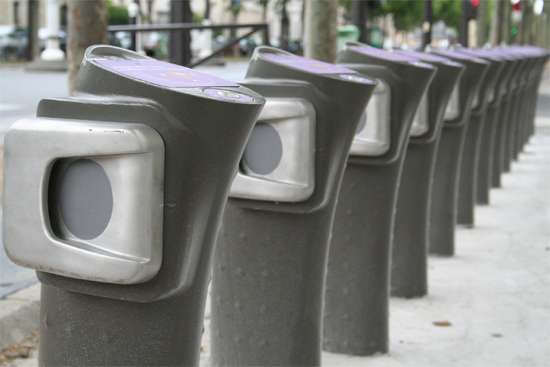
\includegraphics[scale=0.29]{/Users/Juste/Documents/ComplexSystems/CityBikes/Data/images/velib-station-vide}\,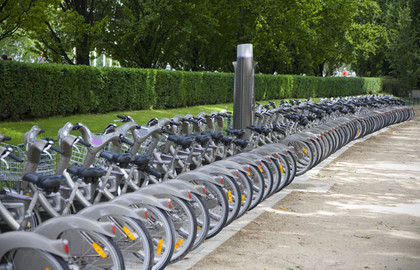
\includegraphics[scale=0.39]{/Users/Juste/Documents/ComplexSystems/CityBikes/Data/images/velibpleine}\caption{Full or empty docking stations in Paris: decrease in the level of
service (source www.velib.paris.fr)}
\end{figure}



\lyxframeend{}\lyxframe{Solutions ?}

\vfill{}

\begin{itemize}
\item Better initial design of the system ? (\cite{lin2011hub,lin2011strategic}).
But at least as complex as transportation predictive models.
\end{itemize}
\vfill{}

\begin{itemize}
\item Optimal management by the operator ? Operational Research give answers
for optimal redistribution (\cite{nair2011fleet,nair2013large}) but
that usually does not solve totally the issues.
\end{itemize}
\vfill{}

\begin{itemize}
\item Poor litterature on user-based models (e. g. \cite{barth2004trb},
but for car-sharing system, for which problems are different). We
want to explore through agent-based modeling impact of some user parameters
on an overall system.
\end{itemize}
\vfill{}



\lyxframeend{}\section{Model description}


\lyxframeend{}\lyxframe{Settings and agents}

\vfill{}

\begin{itemize}
\item Agents: bikers with information $i(b)$ (boolean), tolerated walking
radius $r(b)$ and mean speed $\bar{v}(b)$; docking stations located
in space with current standing bikes $p_{b}(s,t)$ and capacity $c(s)$
\end{itemize}
\vfill{}

\begin{itemize}
\item Euclidian network \textrm{$N=(V,E)$, representing the road network.
Stations are nodes of the network and movement of bikers is embedded
in the trace of $N$ in $\mathbb{R}^{2}$}
\end{itemize}
\vfill{}

\begin{itemize}
\item Scale of the district; we suppose known temporal fields of origin
$O(t)$ and destination $D(t)$ (probabilities of O/D given a trip),
boundaries conditions $N(t)$ as flows (in- and outflows) at fixed
boundaries points
\end{itemize}
\vfill{}



\lyxframeend{}\lyxframe{Temporal Evolution\vfill{}
}

At each time step:\vfill{}

\begin{itemize}
\item Start new travels randomly using $O,D,N$ \vfill{}

\item Make bikers in travel advance of the corresponding distance \vfill{}

\item Finish travels and redirect bikers when needed (see flowchart of bikers
behavior)
\end{itemize}

\lyxframeend{}\lyxframe{Bikers behavior}

\hfill{}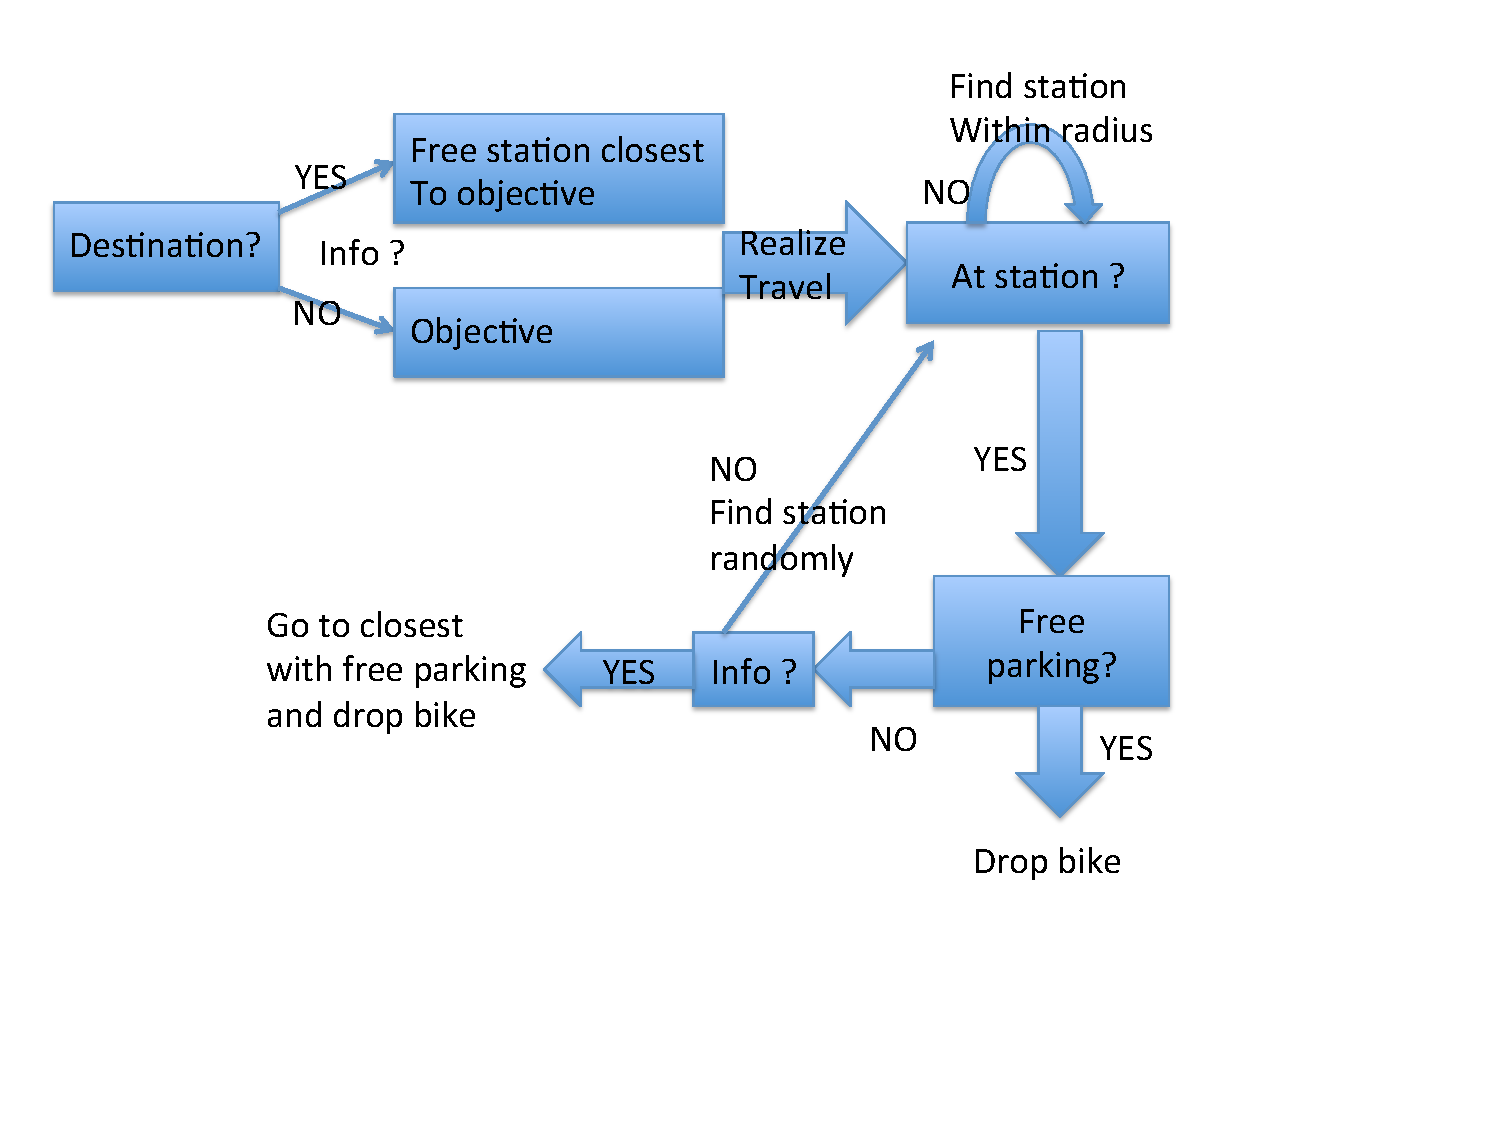
\includegraphics[scale=0.4]{flowchart}\hfill{}


\lyxframeend{}\lyxframe{Evaluation criteria of the level of service}

\textit{\Large Temporal indicators}{\Large \par}
\begin{itemize}
\item Mean load factor $\bar{l}(t)=\frac{1}{\left|S\right|}\sum_{s\in S}\frac{p_{b}(s)}{c(s)}$
\item Heterogeneity of bike distribution (classical spatial heterogeneity
index)
\[
h(t)=\frac{2}{\sum_{s\neq s'\in S}\frac{1}{d(s,s')}}\cdot\sum_{\begin{array}{c}
s,s'\in S\\
s\neq s'
\end{array}}\frac{\left|\frac{p_{b}(s,t)}{c(s)}-\frac{p_{b}(s',t)}{c(s')}\right|}{d(s,s')}
\]

\end{itemize}

\lyxframeend{}\lyxframe{Evaluation criteria of the level of service}

\textit{\Large Aggregated indicators}{\Large \par}

With $\mathcal{T}$ set of travels for a realisation of the system
on a day, $\mathcal{A}$ travels for which an adverse event (full
or empty station) occured and $d_{th}(v)$ ($d_{r}(v)$ ) theoretical
distance (resp. realised) for a travel $v$,
\begin{itemize}
\item Proportion of adverse events $A=\frac{\left|\mathcal{A}\right|}{\left|\mathcal{T}\right|}$
\item Total quantity of detours
\[
D_{tot}=\frac{1}{\left|\mathcal{T}\right|}\cdot\sum_{v\in\mathcal{T}}\frac{d_{r}(v)}{d_{th}(v)}
\]

\end{itemize}

\lyxframeend{}\section{Implementation}


\lyxframeend{}\lyxframe{Parametrisation}

\vfill{}

\begin{itemize}
\item Statistical treatment of real data on 3 month for Paris (time-series
clustering methods) to obtain a ``standard day''; inference of $O,D$
for the area using non-parametric multi-kernel Gaussian estimation.
\end{itemize}
\vfill{}

\begin{itemize}
\item Parameters such as travel distance distribution, mean speed where
taken from the litterature (\cite{o2013mining} ,\cite{nair2013large}
)
\end{itemize}
\vfill{}



\lyxframeend{}\lyxframe{Calibration}

\vfill{}

\begin{itemize}
\item Three remaining parameters: quantity of information, walking tolerance
radius and Gaussian kernel size
\end{itemize}
\vfill{}

\begin{itemize}
\item Simplified calibration procedure (rough reasonable minimum of the
objective) on the mean-square error on load-factors time-series:
\end{itemize}
\[
MSE=\frac{1}{\left|S\right|\left|T\right|}\sum_{t\in T}\sum_{s\in S}(\frac{p_{b}(s,t)}{c(s)}-lf(s,t))^{2}
\]


\vfill{}



\lyxframeend{}\lyxframe{Calibration}

\hfill{}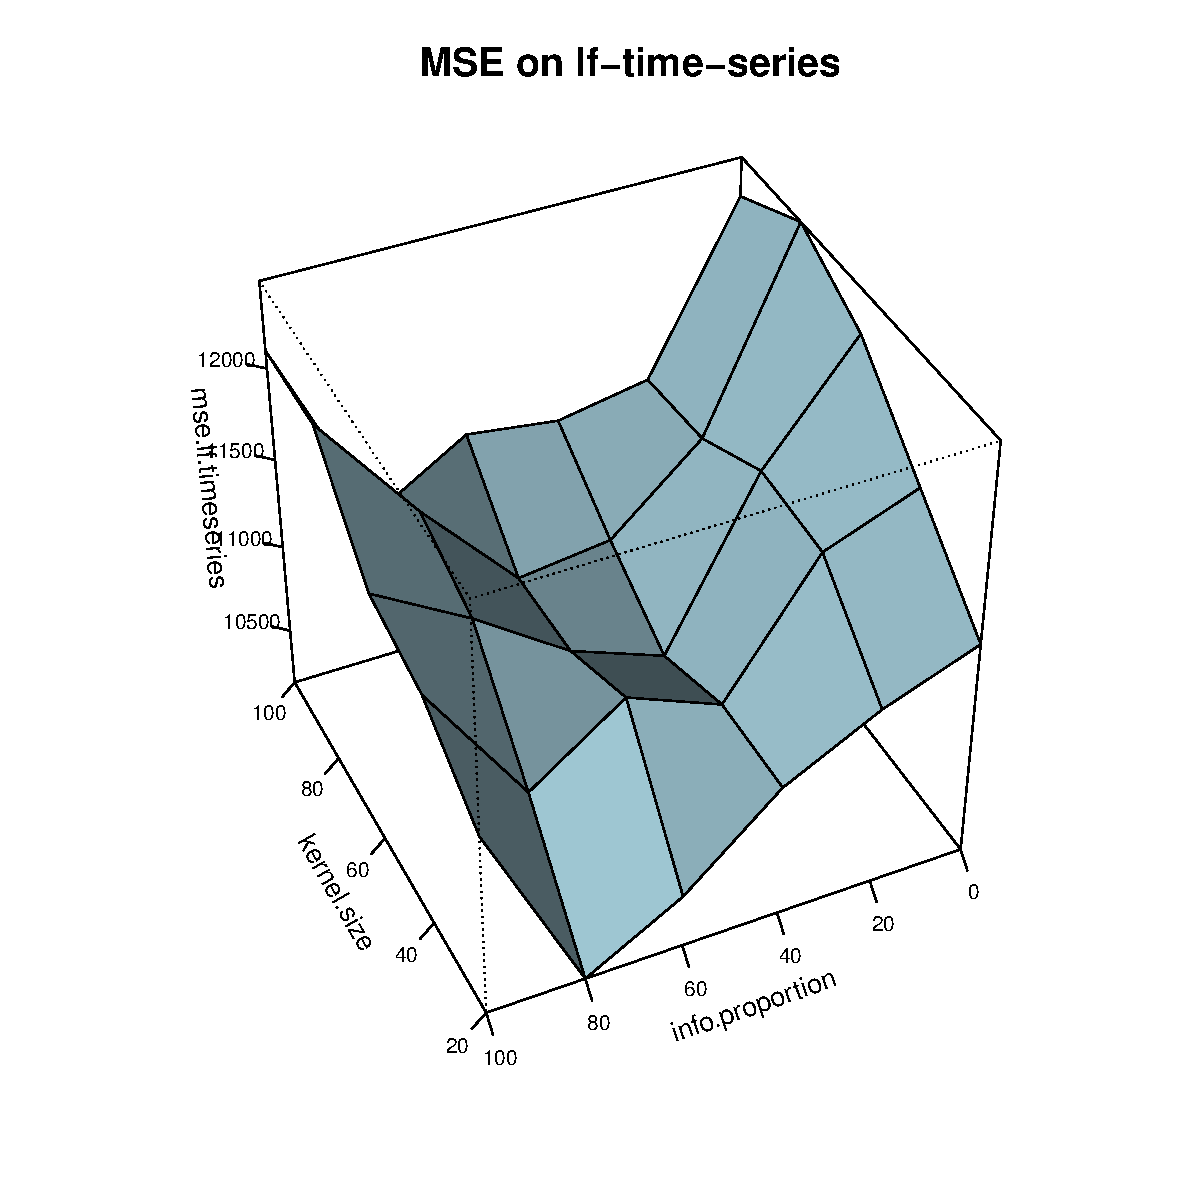
\includegraphics[scale=0.4]{/Users/Juste/Documents/ComplexSystems/CityBikes/Results/Calib/calib3d}\hfill{}


\lyxframeend{}\section{Results}


\lyxframeend{}\lyxframe{Demonstration}

\vfill{}


\hfill{}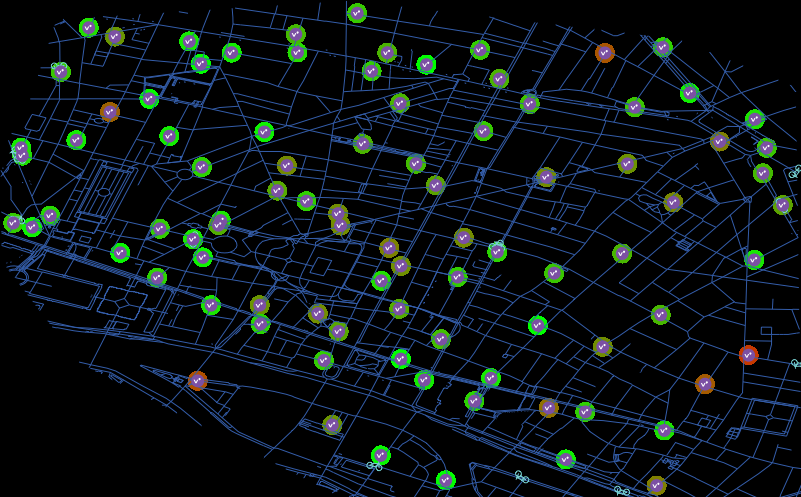
\includegraphics[scale=0.3]{/Users/Juste/Documents/ComplexSystems/CityBikes/Results/Views/running}\hfill{}

\vfill{}


\textit{\large Demonstration of the implementation of the model of
simulation in NetLogo} \vfill{}



\lyxframeend{}\lyxframe{Results: internal robustness}

\begin{figure}
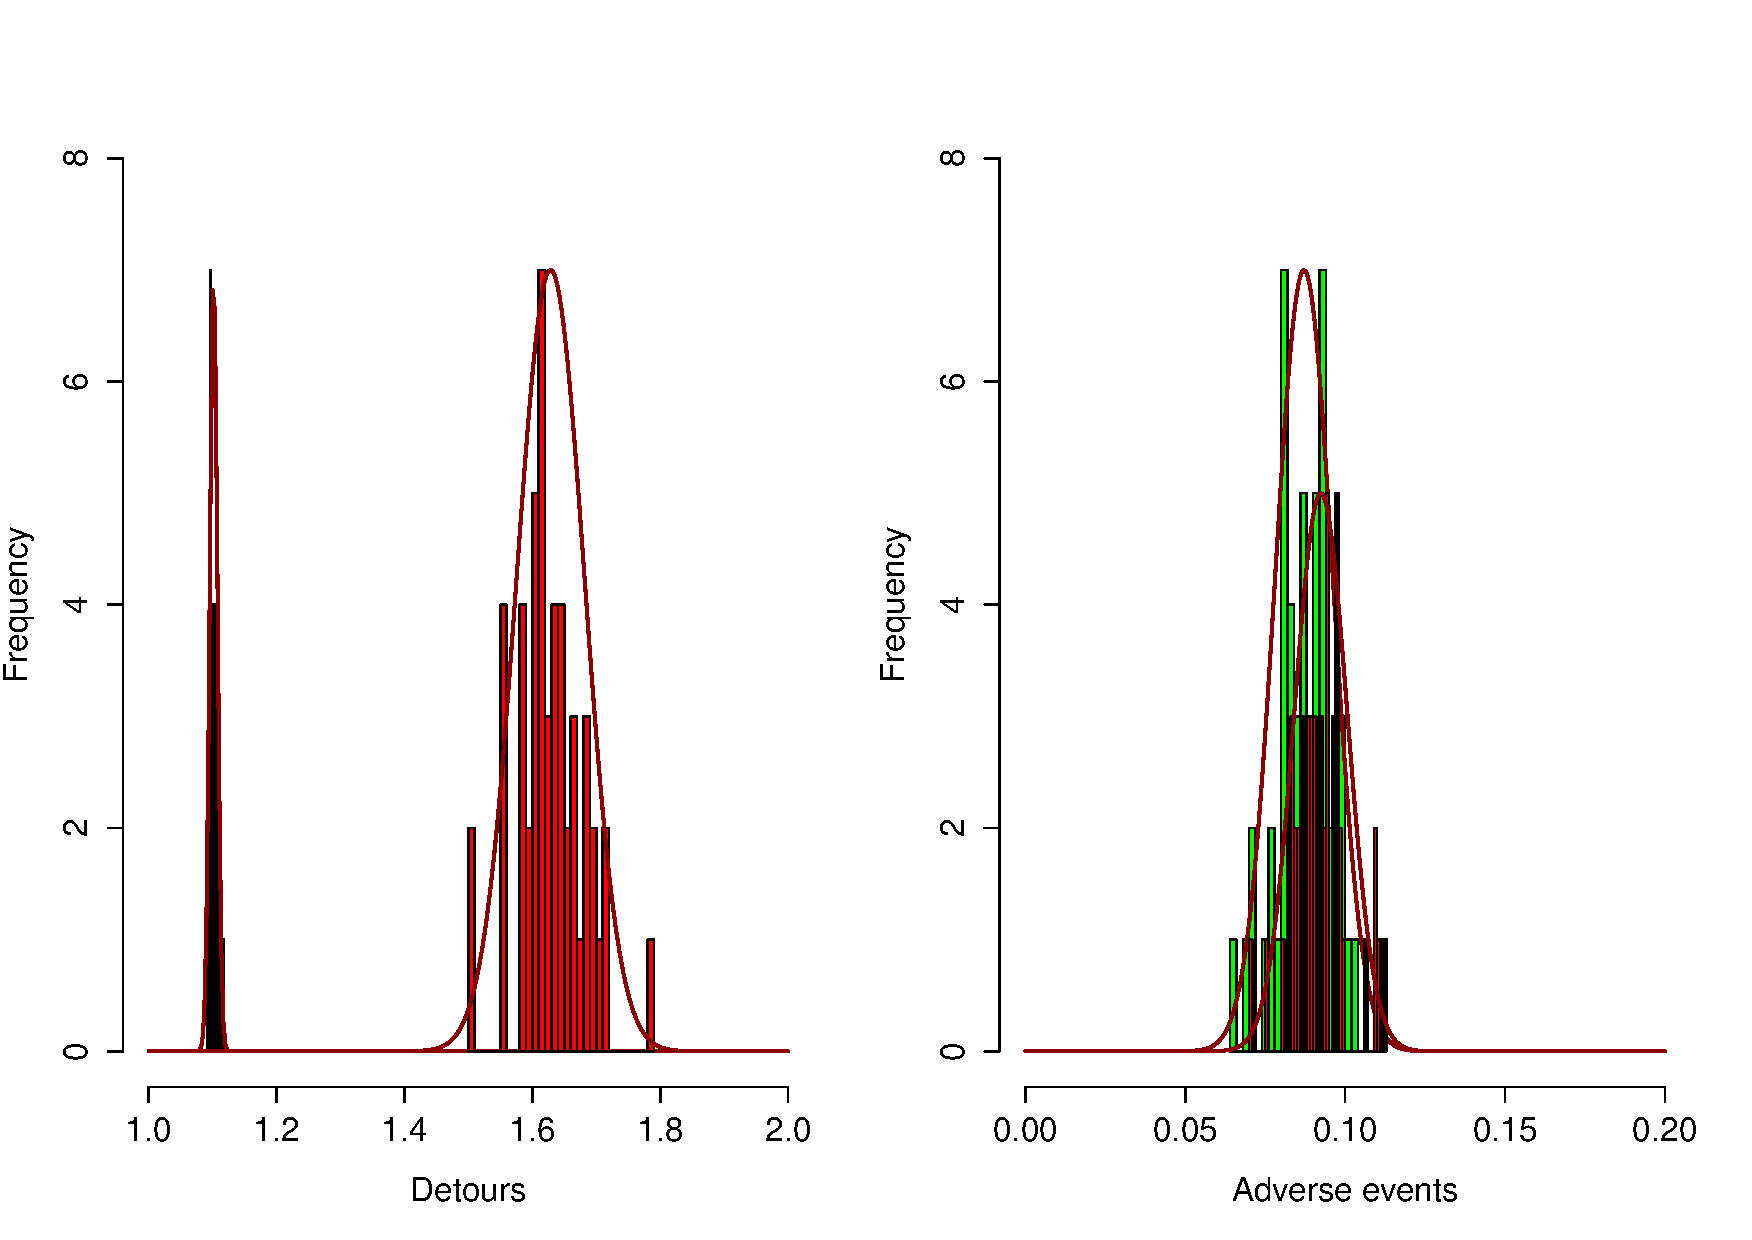
\includegraphics[width=0.6\textwidth]{/Users/Juste/Documents/ComplexSystems/CityBikes/Results/Robustness/histogram}\caption{Statistical analysis of some outputs}
\end{figure}



\lyxframeend{}\lyxframe{Results: ambiguous influence of walking radius}

\begin{figure}
\subfloat[{\footnotesize{} Influence on heterogeneity time-series}]{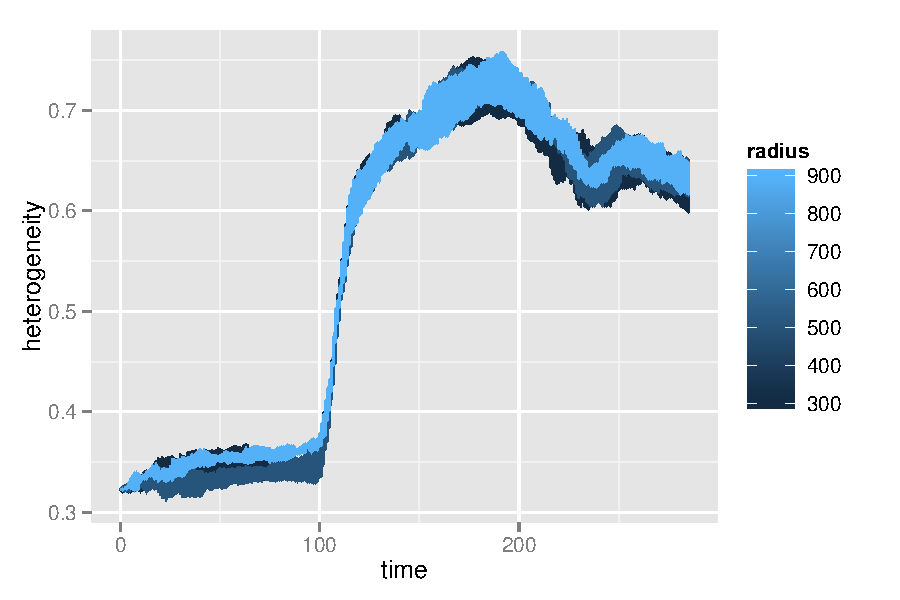
\includegraphics[width=0.5\textwidth]{/Users/Juste/Documents/ComplexSystems/CityBikes/Results/Radius/hetero}

}\subfloat[{\footnotesize Influence on quantity of adverse events}]{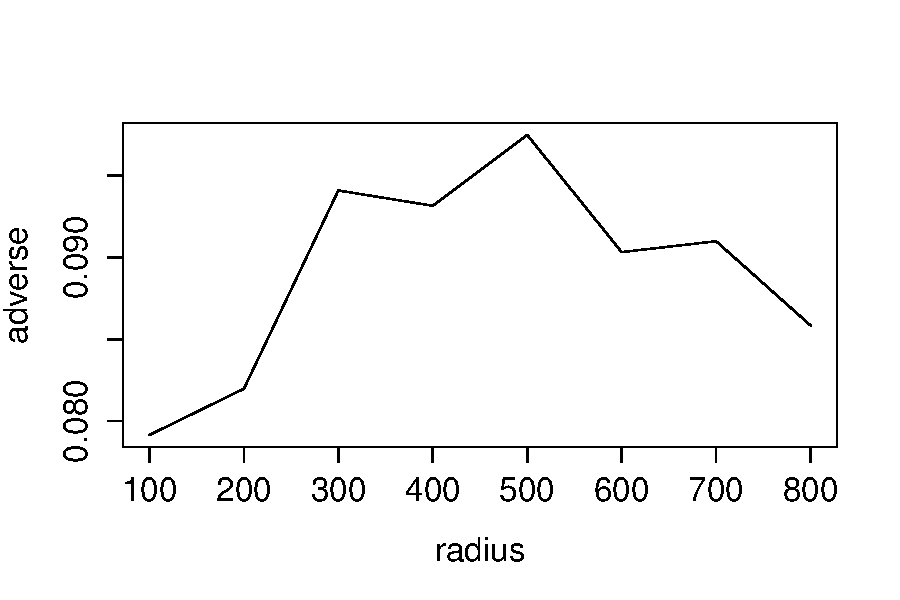
\includegraphics[width=0.5\textwidth]{/Users/Juste/Documents/ComplexSystems/CityBikes/Results/Radius/adverseRadius}

}{\footnotesize{} }\caption{Exploration of the role of walking radius}
\end{figure}



\lyxframeend{}\lyxframe{Results: significant influence of information}

\begin{figure}
\subfloat[{\footnotesize{} Influence on quantity of adverse events}]{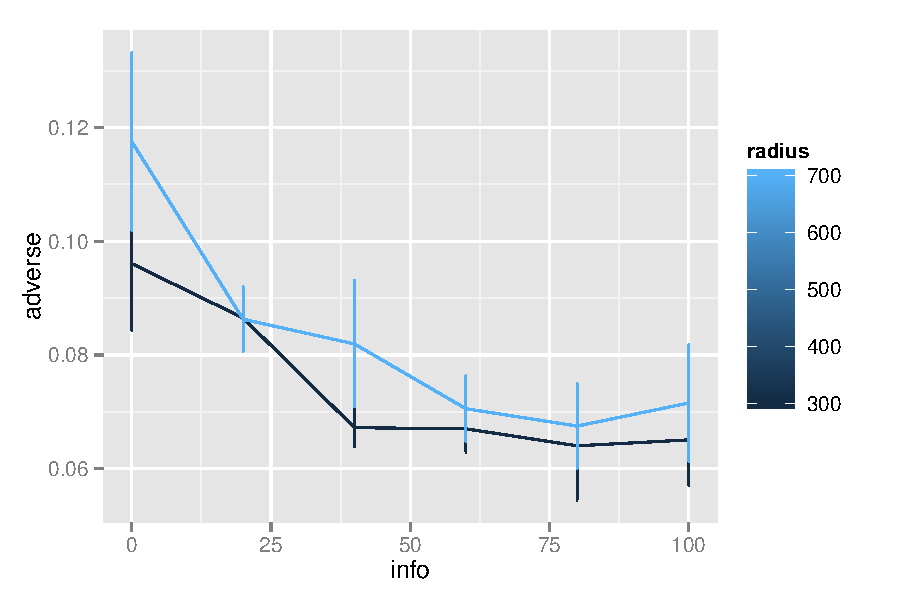
\includegraphics[width=0.45\textwidth]{/Users/Juste/Documents/ComplexSystems/CityBikes/Results/Info/adverse}

}\subfloat[{\footnotesize Influence on quantity of detours}]{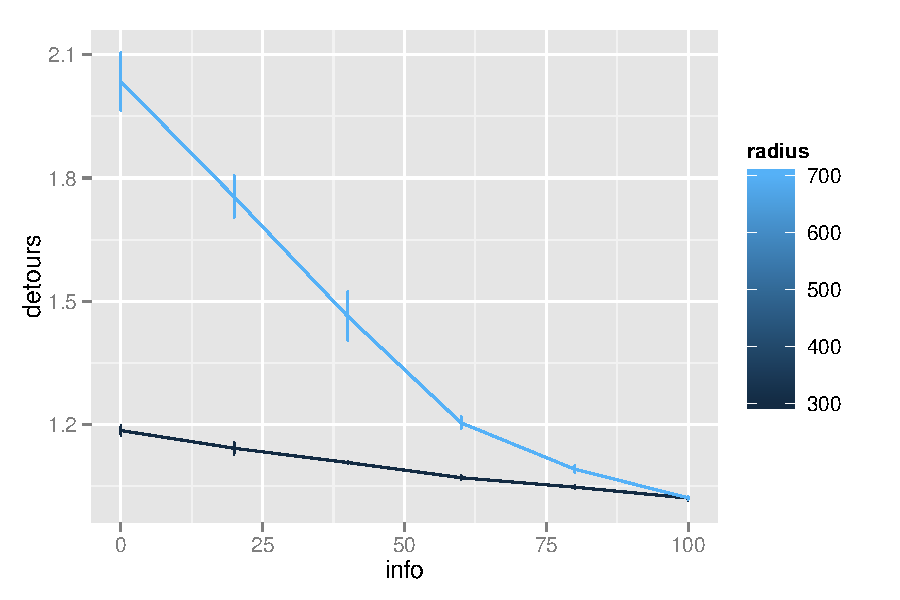
\includegraphics[width=0.45\textwidth]{/Users/Juste/Documents/ComplexSystems/CityBikes/Results/Info/detours}}{\footnotesize{}
}\caption{Exploration of the role of quantity of information}
\end{figure}



\lyxframeend{}\lyxframe{Conclusion}

\vfill{}

\begin{itemize}
\item First step towards a comprehensive bottom-up of that hybrid transportation
system. Parametrisation, calibration and exploration of a simple behavioral
agent-based model \vfill{}

\item Significant qualitative and quantitative results concerning information,
less significant regarding walking radius (suggest deeper exploration
of the relation between topology and users through spatial feedbacks).
\vfill{}

\item Ideas on an online adaptative algorithm for a bottom-up pilotage of
the system, using stations as intelligent agents ? Link between adaptative
intelligent traffic lights and ant algorithms (\cite{monmarche2004algorithmes})
?
\end{itemize}
\vfill{}



\lyxframeend{}

\begin{frame}[allowframebreaks]
\frametitle{References}

\bibliographystyle{apalike}
\bibliography{/Users/Juste/Documents/Cours/ComplexSystemsMadeSimple/project/Biblio/projetCSMS,/Users/Juste/Documents/ComplexSystems/Biblio/BibTeX/global,/Users/Juste/Documents/ComplexSystems/CityBikes/Biblio/bibtex,/Users/Juste/Documents/ComplexSystems/Biblio/Culture/BibTex/culture}


\end{frame}


\lyxframeend{}\lyxframe{Questions}

{\LARGE \hfill{}}{\Huge ?}{\LARGE \hfill{}\hfill{}}{\LARGE \par}


\lyxframeend{}
\end{document}
